\documentclass{beamer}
\usetheme{Madrid}
\usepackage{pgfplots}
\pgfplotsset{compat=1.18}

\title{Modeling Efficiency of Self-Administered Pension Funds in Zimbabwe using an Enhanced Frontier Based Optimization Analysis}
\author{H220021Y}
\institute{Harare Institute of Technology}
\date{2026}

% Remove title from footline, keep author (reg number) and institute
\makeatletter
\setbeamertemplate{footline}{
  \leavevmode%
  \hbox{%
  \begin{beamercolorbox}[wd=.333333\paperwidth,ht=2.25ex,dp=1ex,center]{author in head/foot}%
    \usebeamerfont{author in head/foot}\insertshortauthor
  \end{beamercolorbox}%
  \begin{beamercolorbox}[wd=.333333\paperwidth,ht=2.25ex,dp=1ex,center]{institute in head/foot}%
    \usebeamerfont{institute in head/foot}\insertshortinstitute
  \end{beamercolorbox}%
  \begin{beamercolorbox}[wd=.333333\paperwidth,ht=2.25ex,dp=1ex,right]{date in head/foot}%
    \usebeamerfont{date in head/foot}\insertshortdate{}\hspace*{2em}
    \insertframenumber{} / \inserttotalframenumber\hspace*{2ex}
  \end{beamercolorbox}}%
  \vskip0pt%
}
\makeatother

\begin{document}

\frame{\titlepage}

% ============================================================
% CHAPTER 1: INTRODUCTION
% ============================================================

\begin{frame}
    \frametitle{Statement of the Problem}
    \begin{itemize}
        \item No established optimization-based framework for assessing pension fund efficiency in Zimbabwe
        \item Regulatory oversight primarily emphasises compliance and solvency, not managerial efficiency
        \item In an economy with persistent inflation and financial instability:
        \begin{itemize}
            \item Inefficiency leads to misallocation of long-term savings
            \item Erosion of contributors' retirement benefits
            \item Reduced confidence in the pension system
        \end{itemize}
        \item \textbf{Core gap:} Absence of a rigorous, quantitative evaluation incorporating both managerial performance and scale effects using DEA
    \end{itemize}
\end{frame}

\begin{frame}
    \frametitle{Research Objectives}
    \begin{enumerate}
        \item To evaluate the \textbf{technical efficiency} of self-administered pension funds in Zimbabwe using a Data Envelopment Analysis framework
        \item To \textbf{decompose} overall technical efficiency into pure technical efficiency and scale efficiency components
        \item To \textbf{benchmark} individual pension fund efficiency scores against best-practice peers and rank funds relative to the efficiency frontier
    \end{enumerate}
\end{frame}

\begin{frame}
    \frametitle{Research Questions}
    \begin{enumerate}
        \item Are self-administered pension funds in Zimbabwe technically efficient in utilizing their resources?
        \item To what extent can overall technical inefficiency be decomposed into pure technical and scale efficiency components?
        \item How do self-administered pension funds benchmark against best-practice peers on the efficiency frontier?
    \end{enumerate}
\end{frame}

\begin{frame}
    \frametitle{Significance of the Study}
    \begin{itemize}
        \item \textbf{Academic:} Contributes to limited literature on pension fund efficiency in developing economies; applies frontier-based measurement framework (Kaffash et al., 2020)
        \item \textbf{Methodological:} Demonstrates application of non-parametric optimisation techniques (DEA) reinforcing their relevance for pension fund evaluation
        \item \textbf{Policy:}
        \begin{itemize}
            \item Provides regulators with objective benchmarks beyond compliance indicators
            \item Insights into resource allocation and scale optimisation for fund managers
            \item Contributes to improved retirement income security
        \end{itemize}
    \end{itemize}
\end{frame}

\begin{frame}
    \frametitle{Scope and Assumptions}
    \begin{itemize}
        \item \textbf{Scope:}
        \begin{itemize}
            \item Selected registered and active \textbf{self-administered standalone} pension funds in Zimbabwe (IPEC-regulated)
            \item Five-year study period: \textbf{2018--2022}
            \item Limited to technical efficiency using secondary financial data
            \item NSSA, insured funds, and informal sector arrangements excluded
        \end{itemize}
        \item \textbf{Key Assumptions:}
        \begin{itemize}
            \item Financial statements accurately represent pension fund operations
            \item Selected inputs and outputs adequately capture fund activities
            \item DEA assumptions regarding relative efficiency are satisfied
        \end{itemize}
    \end{itemize}
\end{frame}

% ============================================================
% CHAPTER 3: METHODOLOGY
% ============================================================

\begin{frame}
    \frametitle{Research Design}
    \begin{itemize}
        \item \textbf{Quantitative research design} based on Data Envelopment Analysis (DEA)
        \item DEA: non-parametric linear programming technique measuring relative efficiency of Decision-Making Units (DMUs)
        \item Each pension fund = one DMU
        \item \textbf{Input-output framework:}
        \begin{itemize}
            \item \textbf{Inputs:} Total Assets ($x_1$), Operating Expenses ($x_2$), Total Equity \& Debt ($x_3$)
            \item \textbf{Outputs:} Net Investment Income ($y_1$), Members' Contributions ($y_2$)
        \end{itemize}
        \item All ZWG figures converted to USD-equivalent at the official exchange rate on the financial statement date
    \end{itemize}
\end{frame}

\begin{frame}
    \frametitle{Sample}
    \begin{itemize}
        \item 12 registered self-administered standalone pension funds (DMU1--DMU12)
        \item Satisfies DEA convention: $\geq 3 \times (3 + 2) = 15$ observations at panel level
        \item Funds include: MIPF, POSB Staff, CBZ Bank Staff, Delta Corp, Zimplats, Air Zimbabwe, Econet Wireless, NRZ Staff, Bindura Nickel, Telecel, Innscor Africa, NMB Bank
        \item Source: IPEC annual regulatory reports (2018--2022)
    \end{itemize}
\end{frame}

\begin{frame}
    \frametitle{Seven-Stage Hybrid DEA Framework}
    \begin{enumerate}
        \item \textbf{Variable Selection \& Data Preparation}
        \item \textbf{CCR Model} --- Constant Returns to Scale (CRS) DEA
        \item \textbf{BCC Model} --- Variable Returns to Scale (VRS) DEA
        \item \textbf{Scale Efficiency Computation}
        \[
            \text{SE}_o = \frac{\theta^*_{\text{CRS},o}}{\theta^*_{\text{VRS},o}}
        \]
        \item \textbf{Peer Analysis \& Target Setting}
        \item \textbf{Simar--Wilson Bootstrap Bias Correction} ($B = 2{,}000$)
        \item \textbf{Random Forest Determinant Analysis}
    \end{enumerate}
\end{frame}

\begin{frame}
    \frametitle{DEA Models}
    \textbf{CCR Model (CRS):}
    \[
        \max \; h_o = \frac{\sum_{r} u_r y_{ro}}{\sum_{i} v_i x_{io}}
        \quad \text{s.t.} \quad
        \frac{\sum_{r} u_r y_{rj}}{\sum_{i} v_i x_{ij}} \leq 1, \quad u_r, v_i \geq \varepsilon
    \]
    \vspace{0.3em}
    \textbf{BCC Model (VRS)} adds a free scalar $u_0$ to capture scale effects:
    \[
        \max \; h_o = \frac{\sum_{r} u_r y_{ro} + u_0}{\sum_{i} v_i x_{io}}
    \]
    \begin{itemize}
        \item $h_o = 1$: fund on the efficiency frontier
        \item $h_o < 1$: fund can reduce inputs proportionally
        \item By construction: $\theta^*_{\text{VRS}} \geq \theta^*_{\text{CRS}}$
    \end{itemize}
\end{frame}

\begin{frame}
    \frametitle{Machine Learning Enhancements}
    \begin{itemize}
        \item \textbf{Stage 6 --- Simar-Wilson Bootstrap:}
        \begin{itemize}
            \item Corrects for finite-sample upward bias in raw DEA scores
            \item $B = 2{,}000$ bootstrap pseudo-samples
            \item Produces bias-corrected scores $\hat{\theta}^*_{\text{BIAS}}$ with 95\% confidence intervals
        \end{itemize}
        \item \textbf{Stage 7 --- Random Forest:}
        \begin{itemize}
            \item Replaces Tobit regression for second-stage determinant analysis
            \item Captures non-linear and interaction effects among macroeconomic factors
            \item $T = 500$ trees; hyperparameters tuned via 5-fold cross-validation
            \item Variable importance: MDI and MDA metrics
        \end{itemize}
        \item Implementation: Python (\texttt{scikit-learn}, \texttt{scipy})
    \end{itemize}
\end{frame}

% ============================================================
% CHAPTER 4: DATA ANALYSIS
% ============================================================

\begin{frame}
    \frametitle{Descriptive Statistics}
    \begin{table}
    \centering
    \small
    \begin{tabular}{lrrrr}
    \hline
    \textbf{Variable} & \textbf{Mean} & \textbf{Std Dev} & \textbf{Min} & \textbf{Max} \\
    \hline
    Total Assets ($x_1$, \$m)         & 15.42 & 21.37 & 0.81 & 78.24 \\
    Operating Exp. ($x_2$, \$m)       &  1.18 &  1.53 & 0.05 &  5.31 \\
    Equity \& Debt ($x_3$, \$m)       & 14.09 & 19.84 & 0.71 & 71.63 \\
    \hline
    Net Inv. Income ($y_1$, \$m)      &  1.82 &  2.61 & 0.02 &  9.43 \\
    Members' Contr. ($y_2$, \$m)      &  2.34 &  3.17 & 0.11 & 11.21 \\
    \hline
    \end{tabular}
    \end{table}
    \begin{itemize}
        \item \textbf{High size heterogeneity}: Total assets range from \$0.81m to \$78.24m
        \item Strong inter-input correlations ($> 0.90$): consistent with DEA literature
        \item Right-skewed output distributions: small number of large funds dominate
    \end{itemize}
\end{frame}

\begin{frame}
    \frametitle{CRS Technical Efficiency Results}
    \begin{itemize}
        \item \textbf{4 funds} (33.3\%) consistently achieved full CRS efficiency (score = 1.000):
        \begin{itemize}
            \item DMU1 (MIPF), DMU3 (CBZ Bank Staff), DMU7 (Econet Wireless), DMU11 (Innscor Africa)
        \end{itemize}
        \item Mean CRS efficiency: \textbf{0.639} --- average fund could reduce inputs by $\approx$36.1\%
        \item Notable efficiency decline in \textbf{2020} (avg 0.573): COVID-19 disruptions
        \item Recovery trend: 0.635 (2021) $\rightarrow$ 0.675 (2022)
    \end{itemize}
    \vspace{0.3em}
    Comparison with Greek occupational pension funds (Chrysanthopoulou et al., 2023):
    \begin{itemize}
        \item Greek average CRS: \textbf{0.730} vs Zimbabwe: \textbf{0.639}
        \item Reflects more severe macroeconomic constraints in Zimbabwe
    \end{itemize}
\end{frame}

\begin{frame}
    \frametitle{VRS and Scale Efficiency Results}
    \begin{table}
    \centering
    \tiny
    \begin{tabular}{llrrrl}
    \hline
    \textbf{DMU} & \textbf{Fund} & \textbf{CRS} & \textbf{VRS} & \textbf{Scale} & \textbf{RTS} \\
    \hline
    DMU1  & MIPF            & 1.000 & 1.000 & 1.000 & CRS \\
    DMU2  & POSB Staff      & 0.412 & 0.524 & 0.786 & IRS \\
    DMU3  & CBZ Bank Staff  & 1.000 & 1.000 & 1.000 & CRS \\
    DMU4  & Delta Corp      & 0.589 & 0.732 & 0.804 & IRS \\
    DMU5  & Zimplats        & 0.373 & 0.398 & 0.937 & DRS \\
    DMU6  & Air Zimbabwe    & 0.264 & 0.291 & 0.907 & IRS \\
    DMU7  & Econet Wireless & 1.000 & 1.000 & 1.000 & CRS \\
    DMU8  & NRZ Staff       & 0.728 & 0.874 & 0.833 & IRS \\
    DMU9  & Bindura Nickel  & 0.503 & 0.584 & 0.861 & IRS \\
    DMU10 & Telecel         & 0.318 & 0.327 & 0.972 & DRS \\
    DMU11 & Innscor Africa  & 1.000 & 1.000 & 1.000 & CRS \\
    DMU12 & NMB Bank        & 0.484 & 0.566 & 0.855 & IRS \\
    \hline
    \textbf{Mean} & & \textbf{0.639} & \textbf{0.691} & \textbf{0.913} & \\
    \hline
    \end{tabular}
    \end{table}
    \scriptsize IRS = Increasing Returns to Scale; DRS = Decreasing Returns to Scale
\end{frame}

\begin{frame}
    \frametitle{Scale Efficiency Analysis}
    \begin{itemize}
        \item Mean Scale Efficiency: \textbf{0.913}
        \item \textbf{6 of 8 inefficient funds} operate under Increasing Returns to Scale (IRS)
        \begin{itemize}
            \item Operating \textit{below} most productive scale size
            \item Would benefit from consolidation and asset growth
        \end{itemize}
        \item \textbf{2 funds} exhibit Decreasing Returns to Scale (DRS): DMU5, DMU10
        \begin{itemize}
            \item Operating \textit{beyond} optimal scale threshold
            \item Require operational rationalisation
        \end{itemize}
        \item Supports IPEC's regulatory objective of encouraging pension fund consolidation
    \end{itemize}
\end{frame}

\begin{frame}
    \frametitle{Peer Analysis and Input Slacks}
    \begin{itemize}
        \item \textbf{DMU7 (Econet Wireless)} is the most frequently referenced benchmark --- peer for 4 inefficient funds
        \item DMU1 (MIPF) and DMU3 (CBZ Bank Staff) serve as peers for 3 funds each
        \item \textbf{Dominant slack variable: Total Equity \& Debt ($x_3$)}
        \begin{itemize}
            \item Primary source of over-capitalisation relative to best-practice peers
            \item Consistent with Chrysanthopoulou et al. (2023) findings
        \end{itemize}
        \item Example: DMU5 (Zimplats) must reduce total assets by \$4.52m and equity \& debt by \$5.12m to reach the frontier
        \item Operating expenses show relatively smaller slack --- cost efficiency more readily managed
    \end{itemize}
\end{frame}

\begin{frame}
    \frametitle{CRS vs VRS Efficiency Scores by Fund}
    \begin{tikzpicture}
    \begin{axis}[
        ybar,
        bar width=5pt,
        width=\textwidth,
        height=0.68\textheight,
        ylabel={Average Efficiency Score},
        xtick={1,2,3,4,5,6,7,8,9,10,11,12},
        xticklabels={DMU1,DMU2,DMU3,DMU4,DMU5,DMU6,DMU7,DMU8,DMU9,DMU10,DMU11,DMU12},
        xticklabel style={rotate=45, anchor=east, font=\tiny},
        ymin=0, ymax=1.15,
        ytick={0,0.2,0.4,0.6,0.8,1.0},
        legend pos=north east,
        legend style={font=\footnotesize},
        enlarge x limits=0.05,
    ]
    \addplot[fill=blue!50] coordinates {
        (1,1.000)(2,0.412)(3,1.000)(4,0.589)(5,0.373)(6,0.264)
        (7,1.000)(8,0.728)(9,0.503)(10,0.318)(11,1.000)(12,0.484)
    };
    \addplot[fill=red!40] coordinates {
        (1,1.000)(2,0.524)(3,1.000)(4,0.732)(5,0.398)(6,0.291)
        (7,1.000)(8,0.874)(9,0.584)(10,0.327)(11,1.000)(12,0.566)
    };
    \legend{CRS (CCR), VRS (BCC)}
    \end{axis}
    \end{tikzpicture}
\end{frame}

\begin{frame}
    \frametitle{Distribution of CRS Efficiency Scores by Year (2018--2022)}
    \begin{tikzpicture}
    \begin{axis}[
        ybar stacked,
        bar width=18pt,
        width=\textwidth,
        height=0.68\textheight,
        ylabel={Proportion of Funds (\%)},
        symbolic x coords={2018, 2019, 2020, 2021, 2022},
        xtick=data,
        ymin=0, ymax=105,
        ytick={0,20,40,60,80,100},
        yticklabel={\pgfmathprintnumber{\tick}\%},
        enlarge x limits=0.15,
        legend pos=north east,
        legend style={font=\footnotesize},
    ]
    \addplot[fill=red!60]    coordinates {(2018,41.7)(2019,33.3)(2020,50.0)(2021,33.3)(2022,25.0)};
    \addplot[fill=orange!60] coordinates {(2018,16.7)(2019,16.7)(2020, 8.3)(2021,16.7)(2022,25.0)};
    \addplot[fill=yellow!60] coordinates {(2018, 8.3)(2019,16.7)(2020, 8.3)(2021,16.7)(2022,16.7)};
    \addplot[fill=green!60]  coordinates {(2018,33.3)(2019,33.3)(2020,33.3)(2021,33.3)(2022,33.3)};
    \legend{$<$60\%, 60--80\%, 80--99\%, 100\% (Efficient)}
    \end{axis}
    \end{tikzpicture}
\end{frame}

\begin{frame}
    \frametitle{Bootstrap Bias-Corrected Efficiency Scores}
    \begin{itemize}
        \item Simar--Wilson bootstrap ($B = 2{,}000$) reveals average upward bias of \textbf{0.031 efficiency units}
        \item Bias-corrected mean CRS efficiency: \textbf{0.608} (raw: 0.639)
        \item 95\% confidence intervals confirm genuine efficiency heterogeneity:
        \begin{itemize}
            \item DMU7 (Econet): [0.934, 0.981]
            \item DMU10 (Telecel): [0.267, 0.332] --- non-overlapping
        \end{itemize}
        \item Frontier funds (DMU1, 3, 7, 11) remain statistically distinct from inefficient funds
        \item Addresses the deterministic limitation of standard DEA for policy inference
    \end{itemize}
\end{frame}

\begin{frame}
    \frametitle{Random Forest Determinant Analysis}
    \begin{table}
    \centering
    \small
    \begin{tabular}{lrrl}
    \hline
    \textbf{Predictor} & \textbf{MDI} & \textbf{MDA} & \textbf{Effect} \\
    \hline
    Exchange Rate Volatility   & 0.312 & 0.298 & Negative \\
    Annual Inflation Rate      & 0.287 & 0.271 & Negative \\
    Fund Size (log Assets)     & 0.198 & 0.214 & Positive \\
    Expense Ratio              & 0.112 & 0.108 & Negative \\
    Returns-to-Scale Class.    & 0.054 & 0.067 & Mixed \\
    Fund Age                   & 0.014 & 0.013 & Positive \\
    \hline
    \end{tabular}
    \end{table}
    \begin{itemize}
        \item Model OOB $R^2 = 0.714$: explains $\approx$71.4\% of efficiency variance
        \item Exchange rate volatility + inflation $\approx$ \textbf{56\% of total variable importance}
        \item Macroeconomic environment is the dominant structural constraint
    \end{itemize}
\end{frame}

% ============================================================
% CHAPTER 5: FINDINGS, CONCLUSIONS, RECOMMENDATIONS
% ============================================================

\begin{frame}
    \frametitle{Research Findings}
    \begin{itemize}
        \item \textbf{RQ1 --- Technical Efficiency:} 8 of 12 funds (66.7\%) are technically inefficient; mean bias-corrected CRS = 0.608; average fund could deliver same outputs with $\approx$39\% fewer inputs
        \item \textbf{RQ2 --- Efficiency Decomposition:} Mean VRS = 0.691 vs CRS = 0.639; scale effects account for a non-trivial share of total inefficiency; IRS dominates among inefficient funds
        \item \textbf{RQ3 --- Benchmarking:} DMU7 (Econet Wireless) is the most applicable benchmark; total equity \& debt is the primary excess input; confidence intervals confirm results are statistically robust
    \end{itemize}
\end{frame}

\begin{frame}
    \frametitle{Conclusions}
    \begin{itemize}
        \item Majority of Zimbabwean self-administered pension funds do \textbf{not} operate at the efficiency frontier
        \item Overall inefficiency decomposes into both managerial (pure technical) and structural (scale) components
        \item IRS among 6 of 8 inefficient funds confirms that \textbf{consolidation} is a priority policy action
        \item Exchange rate volatility and inflation are the \textbf{dominant macroeconomic constraints} on efficiency
        \item Existence of 4 frontier-efficient funds within the same environment confirms that \textbf{efficiency improvement is achievable}
    \end{itemize}
\end{frame}

\begin{frame}
    \frametitle{Recommendations}
    \begin{itemize}
        \item \textbf{For Fund Managers:}
        \begin{itemize}
            \item Adopt peer benchmarking using DMU7 and DMU1 as best-practice references
            \item Rationalise asset and capital structures to reduce equity \& debt slack
        \end{itemize}
        \item \textbf{For IPEC:}
        \begin{itemize}
            \item Institutionalise DEA-based efficiency benchmarking in annual supervisory reporting
            \item Facilitate voluntary consolidation of small IRS-classified funds
            \item Enforce consistent reporting templates for DEA input--output variables
        \end{itemize}
        \item \textbf{For National Policymakers:}
        \begin{itemize}
            \item Prioritise macroeconomic stabilisation (exchange rate and inflation management) as a pension sector efficiency prerequisite
            \item Develop multi-pillar architecture to reduce sector concentration risk
        \end{itemize}
    \end{itemize}
\end{frame}

\begin{frame}
    \frametitle{Prototype Update}
    \begin{itemize}
        \item The prototype decision-support tool developed alongside this research now incorporates a \textbf{user interface}
        \item The interface allows fund managers and regulators to input DEA variables and view efficiency scores interactively
        \item \textbf{Backend logic} for running the DEA and Random Forest models is currently under development
        \item The goal is a fully integrated system enabling real-time efficiency benchmarking for Zimbabwean pension funds
    \end{itemize}
\end{frame}

\begin{frame}
    \frametitle{Contribution to Knowledge}
    \begin{itemize}
        \item \textbf{First} DEA efficiency study of self-administered pension funds in Zimbabwe
        \item Introduces a \textbf{seven-stage hybrid DEA--machine learning framework} transferable to other emerging market pension studies
        \item Demonstrates feasibility of frontier analysis using \textbf{secondary regulatory data} in data-scarce environments
        \item Expands comparative evidence on pension fund efficiency in \textbf{low- and middle-income countries}
    \end{itemize}
\end{frame}

\begin{frame}
    \frametitle{Future Research Directions}
    \begin{enumerate}
        \item \textbf{Longitudinal extension} --- expand panel to 10+ years
        \item \textbf{Environmental DEA models} (Banker \& Natarajan, 2008) --- integrate macro covariates directly into the LP
        \item \textbf{Network DEA} --- decompose efficiency into investment management vs. administration sub-processes
        \item \textbf{Cross-country SADC comparison} using meta-frontier DEA
        \item \textbf{Dynamic DEA \& Malmquist indices} --- distinguish frontier shifts from catch-up effects
    \end{enumerate}
\end{frame}

\begin{frame}
    \frametitle{References}
    \tiny
    \begin{itemize}
        \item Banker, R.D., Charnes, A. \& Cooper, W.W. (1984). \textit{Management Science}, 30(9), 1078--1092.
        \item Barr, N. \& Diamond, P. (2016). \textit{Reforming Pensions}. Oxford: OUP.
        \item Barros, C.P. \& Garcia, M.T.M. (2006). \textit{Risk Management and Insurance Review}, 9(2), 165--188.
        \item Breiman, L. (2001). \textit{Machine Learning}, 45(1), 5--32.
        \item Charnes, A., Cooper, W.W. \& Rhodes, E. (1978). \textit{European Journal of Operational Research}, 2(6), 429--444.
        \item Chrysanthopoulou, X., Mavrommati, A. \& Migdalas, A. (2023). \textit{Operational Research}, 23(66), 1--30.
        \item IPEC (2023). \textit{Annual Report 2022}. Harare: IPEC.
        \item Kaffash, S. et al. (2020). \textit{European Journal of Operational Research}, 284(3), 801--813.
        \item OECD (2022). \textit{Pension Markets in Focus 2022}. Paris: OECD Publishing.
        \item Simar, L. \& Wilson, P.W. (2007). \textit{Journal of Econometrics}, 136(1), 31--64.
        \item Verberi, C. \& Kaplan, M. (2026). \textit{Journal of Financial Regulation and Compliance}, 34(1), 45--67.
        \item World Bank (1994). \textit{Averting the Old Age Crisis}. Oxford: OUP.
    \end{itemize}
\end{frame}

\begin{frame}
    \frametitle{Questions}
    \centering
    \Huge{Thank You}
\end{frame}

\end{document}
